\subsection{Definitionen}
\begin{itemize}
	\item \textbf{Pervasive Computing}
	\begin{itemize}
		\item Pervasive Computing $\approx$ Ubiquitous Computing
		\item pervasive = \textit{alles durchdringend}
		\item IBM-Definition: \glqq Convenient access, through a new class of appliances, to relevant information with the ability to easily take action on it when and where you need\grqq
		\item Beispiel: Smartphones $\rightarrow$ relativ neue Technologie, daher viel höhrere Dynamik in der Entwicklung als beim Desktop. 
		\item Implizite Interaktionen: Gerät reagiert implizit auf User-Aktivität (insbesondere bei Smart Homes), jüngere lernen das besser (je älter man wird, desto mehr muss man anhand von Bezügen zu bereits Gelerntem/Metaphern lernen)
	\end{itemize}
	\item \textbf{Human Adopted Production}
	\begin{itemize}
		\item Comber and Maltby (1997) found that both overly simple and overly complex computing interfaces were low in usability 
		\item Wie kann man den User \glqq bei Laune halten\grqq ?\\
	 	$\rightarrow$ Die aktuell erfahrene Komplexität muss im Mittelmaß sein\\
	 	$\rightarrow$ Lernsysteme greifen per GSR Stress Level des Users ab und tunen dementsprechend das Lernsystem\\
	 	$\rightarrow$ kognitive Paramater sind sehr individuell
		\begin{figure}[h!]
			\centering
			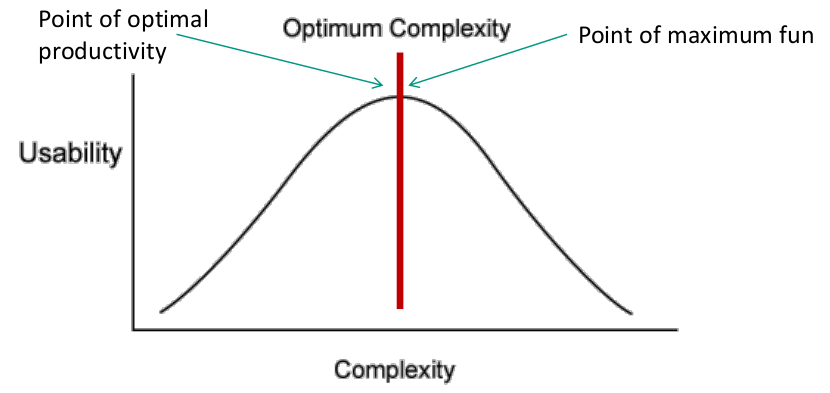
\includegraphics[width=.4\textwidth]{img/ch01_HAP.png}
			\caption{Human Adopted Production}
			\label{HAP}
		\end{figure} 
	\end{itemize}
	\item \textbf{Mensch-Maschine Interaktion}
	\begin{itemize}
		\item Important part of Pervasive Computing, e.g. Mobile Phone interfaces
		\item Pervasive Computing Technology produces now most/all innovative human machine interfaces, e.g. augmented reality glasses
	\end{itemize}
\end{itemize}
\subsection{Anwendungen}
\begin{itemize}
	\item Reprogramming Senses: Proxmity Helmet (mit Arduino) $\rightarrow$ wird nach einer Weile zum Gefühl, so kann man neue Sinne erschaffen
	\item Augmented Reality, Mobile Computing User Interface Software Design
	\item Wearable Thermography: detektiert Überbelastung bei Sport...
	\item Ubiquitous Sensing: Lobster House, Büro welches sich nach Sonne dreht, jeder Quadratmeter individuell klimatisierbar
\end{itemize}



